\chapter{Related Work} % English: Related Work
\label{chap:relwork}

Much work has been done evaluating \ac{RPL} and its repair process.
In the following, a brief introduction to \ac{RPL} will be given, then previous research concerning the general performance of the protocol will be presented.
After this, an overview of the sources of unreliability in \ac{WSN} follows and resetting nodes as a factor for network disruption are considered in more detail, before work is presented discussing the effects of the resulting transient node failures in more detail.
From the literature, extensions to \ac{RPL}, that may help to improve protocol reliability and network lifetime, will be presented, including optimizing the \ac{OF} for network lifetime, improving the formation of network paths, implementing fairer broadcast suppression, using intrusion detection systems, adding trust and authenticity and storing routing information persistently.

\section{Introduction to RPL}

\ac{RPL} as defined in \cite{rfc6550} is a routing protocol for \acp{LLN} that provides energy efficient networking for resource-constrained devices in networks where interconnects are expected to be bidirectional, but may have low data rates, high error rates and be unstable.
In \ac{RPL}, nodes self-organize to form a \ac{DODAG}, where the node with the lowest rank is the destination of and the root of the \ac{DAG}.
Such a \ac{DODAG} is displayed in \autoref{fig:dodag}.

The bootstrapping process defines how nodes may join the network by selecting a parent and how to globally or locally repair the network when necessary.
Each node emits \ac{DIO} messages targeted at all nodes in transmission range.
These messages advertise the presence of a node, its affiliation with an existing \ac{DODAG}, the current routing costs and related metrics.

A joining node may receive these messages and select a parent in the \ac{DODAG}
based on the received rank and routing costs, but must not select a node with a rank lesser than its current.
The separation of the route metric from the forwarding process is an important characteristic of \ac{RPL} as the function that is used to calculate the route metric, the \ac{OF}, can be exchanged to form \acp{DODAG} based on different characteristics.

\begin{figure}[h]
  \centering
  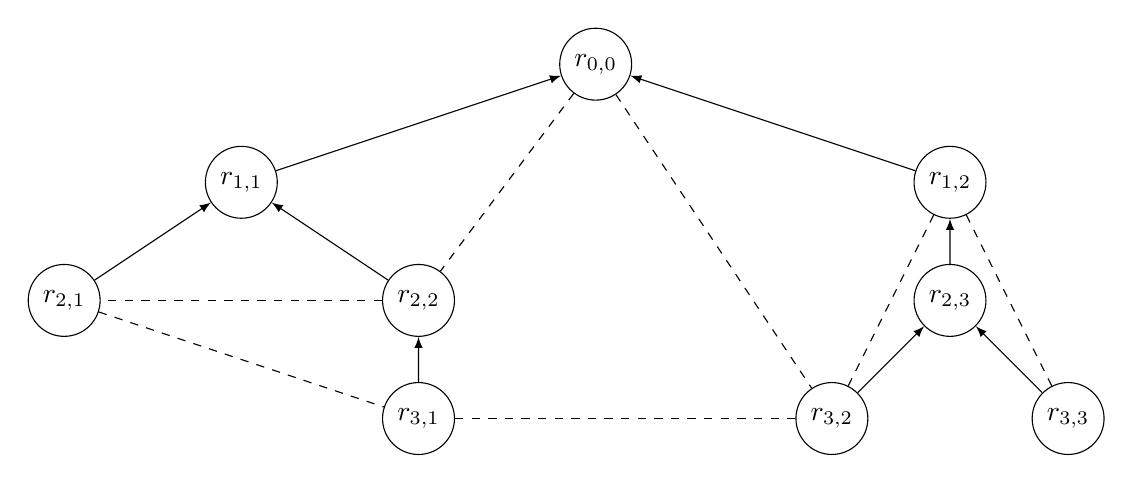
\begin{tikzpicture}[edge from parent/.style={draw,latex-},
      every node/.style={circle,draw},level/.style={sibling distance=90mm/#1}]
    \node (s) {$r_{0,0}$}
    child { node {$r_{1,1}$}
      child { node (d) {$r_{2,1}$}}
      child { node (a) {$r_{2,2}$}
        child { node (f) {$r_{3,1}$} }
      }
    }
    child { node (c) {$r_{1,2}$}
      child { node {$r_{2,3}$}
        child { node (b) {$r_{3,2}$} }
        child { node (e) {$r_{3,3}$} }
      }
    };
    \path (s) edge[dashed] (a);
    \path (s) edge[dashed] (b);
    \path (c) edge[dashed] (b);
    \path (a) edge[dashed] (d);
    \path (c) edge[dashed] (e);
    \path (d) edge[dashed] (f);
    \path (f) edge[dashed] (b);
  \end{tikzpicture}
  \caption{\acf{DODAG}}
  \label{fig:dodag}
\end{figure}

\section{Protocol Performance}

One of the main goals of this work is to evaluate the performance of \ac{RPL} when dealing with transient node failures.
Much research has already been done concerning the general performance of \ac{RPL}.

An extensive survey of energy efficient routing protocols is presented in \ac{WSN} \cite{pantazis2013energy}.
They classify protocols into four main categories, what their forwarding descisions are based on: network structure, communication mode, topology based and reliable routing.
\ac{RPL} is listed as as a reliable routing protocol and further subcategorized as a multipath-based protocol.
As an advantage they list low energy consumption, as a drawback that it only supports unicast traffic.
The scalability is rated as good, as is mobility and robustness.

The effectiveness and performance of \ac{RPL} has been evaluated in many publications \cite{rfc6687,accettura2011performance,korte2012study,ali2012performance,banh2015performance}.
In \cite{rfc6687}, the authors studied \ac{RPL} both in test networks of varying sizes and in simulations.
For the simulations, the link failure model and the network topology have been derived from measurements gathered from real-life deployments.
Simulations were performed using the \emph{OMNet++} \cite{varga2008overview} network simulator.
The authors measured path quality, routing table size, delay bounds, control overhead and connectivity loss.
The study does not directly consider network lifetime and energy consumption as a metric, but results where obtained pertaining to the scalability and performance under realistic scenarios.
It has been found, that \ac{RPL} scales well to very large topologies, provides near optimum path quality, neglible control overhead, and meets desired delay and convergency requirements for the given scenarios.
They also find, that with \ac{RPL} it is possible to tradeoff routing stability for less control overhead and thereby increase network lifetime.

A detailed study of \ac{RPL}, with a range of different parameter settings, as well as a comparison of the OF0 \cite{rfc6552}, which tries optimize for connectivity, and the \ac{ETX}-based \acp{OF} can be found in \cite{ali2012performance}.
Observations where made using the \emph{Cooja} \cite{osterlind2006cross} network simulator for \emph{Contiki}, energy usage has been measured using \emph{Powertrace} \cite{dunkels2011powertrace}.
Results hint to the importance of the settings for the Trickle timer for resource utilisation and the measured parameters.
The \emph{ContikiMac} \cite{dunkels2011contikimac} duty cycling is also found to be beneficiary to energy efficiency.
The findings also include results concerning network latency, delivery ratio, convergence time, control overhead and the energy consumption, using OF0 and \ac{ETX} respectively.
The tendency of node failures to be frequent and often transient is remarked at one point, but the effects were studied explicitly.

In \cite{korte2012study} the \ac{RPL} repair process is studied in more detail.
They evalutate a limited test network using the \emph{Contiki} \ac{RPL} implementation and studied the effect of node failures on the formation of the \ac{DODAG} before it undergoes local or global repair.
Here, the duration of the repair process and its individual steps are recorded and evaluated, as well as the results.
They were also able to confirm that the repaired \ac{DODAG} still matches the optimal \ac{DODAG} created by the \ac{OF}.
Although \cite{korte2012study} did not consider the additional energy usage from node failure, they find that most of the time it takes to recover from failure is spent on detecting a failed node, which may be useful when optimising the energy efficiency of the recovery process.
They also hint at the ability of \ac{RPL} to make use of an \ac{OF} that uses the remaing energy of a node as a metric.
This may help to balance energy consumption inside the network and thereby increase overall network lifetime.

While multiple other studies find that simulations of \ac{RPL} and experimental
results are largely consistent, Korte et al. \cite{korte2012study} measured a noticeable difference when comparing experimental results to simulations made in the network simulator \emph{NS2}\footnote{\url{https://www.isi.edu/nsnam/ns/}}.
They also remark that, for some situations, the time at which certain protocol messages must be send is underspecified in \ac{RPL}.
Depending on implementation details, these may lead to the creation of loops, which make it necessary to initiate a global repair of the \ac{DODAG}.
Additionally, the \ac{NUD} employed in \ac{RPL} may not be indicative for a loss of connectivity if higher layer protocols that function across longer than one hop paths, like \ac{TCP}, are used as an indication of connectivity.

When it comes to the effects of failing nodes, most research focuses on the performance of the local and global repair processes, but either it does not consider the possibility of transient node failure, or neglects the effects on the network lifetime from the resulting increased energy usage.

\section{Sources of Unreliability in WSN}

When evaluating networks with failing nodes, it is important to differentiate
the underlying cause for the failure, since failures from different causes may
exhibit different behavior concerning frequency, duration, and intensity of the
fault. As an example, while an error in programming for an edge-case may result
in only a single node restart, failures from overheating may be result in many
consecutive restarts. \cite{boano2013hot,boano2010impact}

The sources of unreliability in \ac{WSN} can be classified into those where an active attacker is involved and those where unreliable behavior is caused by passive environmental conditions.

%In energy constrained devices such as wireless sensor nodes, duty cycling is an important mechanism for conserving energy.
%One example of this is \emph{ContikiMAC} \cite{dunkels2011contikimac}, where the radio is only enabled for certain intervals of time.
When undervolting a sensor node, components of the nodes are run outside of their specified voltage range.
While this presents an interesting opportunity to increase the lifetime of \acp{WSN}, it may also increase the error rate of components and therefore may cause unpredictable behavior or even temporary node failure \cite{kulau2015undervolting}.
An implementation of undervolting for \ac{WSN} has been done by \cite{kulau2016idealvolting}.
They use supervised learning to adapt the voltage levels for individual nodes based on clock speed, temperature variations and differences in the manufacturing process.
This made it possible to prolong the lifetime of the network by more than 40\%.

Besides undervolting, there are many other factors in \ac{WSN} that may cause temporary node failure, such as temperature variations \cite{boano2010impact,boano2013hot,reynolds1974thermally}, programming errors and faulty components.

An overview of common active attacks against \acp{WSN} is presented by Karlof et
al.\cite{karlof2003secure}.
Surveyed modes of attack include: spoofed, altered, or replayed routing information, selective forwarding, sinkhole attacks, Sybil attacks, wormholes, HELLO flood attacks and acknowledgement spoofing.
As an ad-hoc, hierarchical routing protocol, \ac{RPL} is generally vulnerable against all of the described attacks.

\section{Effects of Transient Node Failures}

One attack not explicitly mentioned in \cite{karlof2003secure} is based on repeatedly restarting nodes as a possible attack vector.

Depending on the topology of the network, a single restarting node may cause transient node failures in other parts of the network and significantly increase the overall energy consumption of the network \cite{kulau2017energy}.
This may also be exploited by an active attacker.
Attacker controlled nodes integrate with the network, possibly using wormholing, in a way that as many paths as possible include the nodes as their parents.
The nodes then fail for a short time and subsequently restart.
By coordinating the timing and spacing of the restarts, an attacker repeatedly forces the network to repair itself.
As this behavior may also be triggered by malfunctioning nodes, such an behavior
may also be triggered accidentally.

In \cite{kulau2017energy}, the energy impact of single node restarts when using \ac{RPL} is studied in detail.
Experiments were done using the \emph{Cooja} network simulator and then compared to a reference simulation without resetting nodes.
Both the effect of single node restarts and multiple node restarts were investigated on a binary tree topology and for a meshed network, where each node can have more than one parent.
They discovered that a single node restart leads to an increased energy consumption of up to 20\% for the restarting node and its direct neighbors.
To remedy the effect of passive node failure, they suggest optimising \ac{RPL} parameters and keeping persistent information across node restarts, while, in case of an active attacker an \ac{IDS} would be more applicable.

\section{Extensions to RPL}

While \ac{RPL} is comparatively easy to implement, it has some weaknesses when it comes to mobility, energy consumption and packet delivery rates.
Some research that was done to extend and improve the protocol is presented here.

\subsection{Objective Functions}

An \ac{OF} is the function by which \ac{RPL} selects a parent in the \ac{DODAG} based on a metric like end-to-end delay, energy usage or delivery probability.
Since, in \ac{RPL}, the choice of \ac{OF} is independent of the forwarding mechanism, it is possible to substitute an \ac{OF} that produces a \ac{DODAG} that will be less effected by certain types of failure conditions.
A network can even have multiple \acp{DODAG}, that each can be optimized for different use cases.
Kamgueu et al. Kamgueu et al. \cite{kamgueu2013energy} implemented an \ac{OF} that uses the remaining energy of a candidate parent as a metric.
This way it is possible to create a \ac{DODAG} that distributes energy usage within the network more evenly and therefore increases network lifetime.
As opposed to computing the total energy level of a path, the costs for a path is the minimum energy level of any node in the path.
The \ac{OF} is evaluated using the \emph{Cooja} simulator for a network of 20 nodes.
They where able to increase network lifetime by around 14\% compared to a network using the \ac{ETX}-based \ac{OF}.
At the same time, the energy-based \ac{OF} achieved around 3\% worse delivery ratio compared to the \ac{ETX}-based \ac{OF}.
They note that future work would be needed to combine \ac{ETX} and energy-based \ac{OF}, to obtain both long network lifetime and a stable network.

\subsection{Coronal RPL}

In \cite{gaddour2014co} \ac{Co-RPL} is proposed as an an extension to \ac{RPL} and evaluated.
Co-\ac{RPL} makes use of the Corona mechanism \cite{olariu2006design} to help in the selection of a parent router and includes a procedure for reducing packet loss in case of a failing parent node.
It has been found that, in specific scenarios, \ac{Co-RPL} reduces end-to-end delay by up to 2.5 seconds, packet loss by up to 45\% and energy consumption by up to 50\%.

\subsection{Trickle Timer}

The time and therefore energy needed for a failed node to re-join the network is also influenced by the behavior of its \emph{Trickle} timer \cite{levis2004trickle}.
For \ac{RPL}, such a timer, based on the number of messages received during a sensing interval, regulates if the sender may send messages after the sensing interval.
Since the behavior of the \emph{Trickle} timer for networks of more than one node is inherently non-deterministic, it is possible that the share of sending time each node gets may be unfair \cite{vallati2013trickle}.
This in turn can result in less than optimal route selections when sensing for possible parents during the bootstrapping process.
\emph{Trickle-F} \cite{vallati2013trickle} is an attempt at adding fair broadcast suppression to the \emph{Trickle} algorithm.
Evaluations have shown its validity and that it was possible to obtain more efficient routes with same power consumption as the original algorithm.

\subsection{Intrusion Detection Systems}

As a method for recognizing and preventing large scale attacks on \ac{WSN}, different \acfp{IDS} implementations have been discussed in the literature \cite{le2011specification,raza2013svelte,kasinathan2013denial}.
These approaches have some considerable disadvantages for \ac{WSN}.
First, \ac{IDS} are most efficient if all information is available at a central location.
This requires a considerable traffic flow from each node to a central sink node, which consumes additional energy and therefore reduces network lifetime.
Additionally, nodes closer to the sink node will see more traffic than nodes closer to a leaf of the \ac{DODAG}, which again reduces total network lifetime.
For the node that processes the collected data, a connection to the power mains and additional storage and processing capabilities may be required.
As a consequence of misbehavior, nodes may be prohibited from accessing the network in certain ways.
This in turn requires that other nodes can be provisioned with rules that facilitate such penalties, which, depending on the network state, may not always be given and could be prevented by an active attacker using blackholing attacks.
In this case a distributed algorithm would appear to be more promising.

\subsection{Authentication and Trust}

In \cite{kantert2016combining} an approach for combining trust and \ac{ETX} is demonstrated, that improves the robustness of \ac{WSN} against unreliable or intentionally malicious nodes.
This technique also has been shown to reduce the impact of nodes that repeatedly employ selective forwarding.
Since a repeatedly failing node may also be interpreted as a node that selectively drops packets, it is possible that this will also be detected by this method.

One problem of security in \ac{WSN} is that, because of the limited capabilities of the nodes, message authenticity is often not implemented, which makes the network susceptible to spoofed, altered or replayed routing information \cite{karlof2003secure}.
If the network was be protected against spoofed messages, it would be considerably more difficult for an active attacker to impersonate nodes or create virtual nodes, that take part in attacks on the network.
An implementation of message authenticity and protection against replay attacks can be found in \cite{perazzo2017implementation}.
The authors show that their protection against replay attacks has a considerable negative impact on network formation time, while the message authenticity and encryption only had a modest impact on performance.

\subsection{Persistent Routing Information}

Another promising approach for hardening \ac{RPL} against transient node failures is to reduce the time the bootstrapping process takes by saving some of the state of the \ac{RPL} implementation between node restarts and restoring it after the node has failed.
An implementation of this approach has been created for \emph{Contiki\ac{RPL}} \cite{mueller2017}.
Multiple new problems arise from this approach: The implementation has to guarantee that the saved state remains consistent, even if the node fails while still editing the saved state, and the node needs to be able to decide if a restored state still remains valid.

To solve the problem of data integrity, the implementation constructs a checksum for the stored data and stores it along with the \ac{RPL} state.
On each node, the implementation keeps a clock that describes the recentness of the saved information.
From the clock, the \ac{DODAG} ID, instance ID and the version number of the \ac{DODAG} a \ac{UID} is computed and send alongside other information as part of the \ac{DIO} messages.
Joining nodes receive these \acp{UID}, and can use them to decide if the state of the surrounding network has diverged from the state they have stored before.
Another issue is that the write operations cause additional energy usage.
This issue has been addressed by reducing the number and frequency of writes by directly accessing the device driver instead of relying on the file system.

The evaluation is done using simulations in the \emph{Cooja} network simulator.
Only two topologies were evaluated, a binary tree topology and a meshed star topology, similar to \cite{kulau2017energy}.
The energy overhead of the hardened implementation was measured and compared against the same network using default \emph{Contiki\ac{RPL}} and without using the UID.
Networks without failing nodes and with a repeatedly failing node have been simulated, as well as multiple clock intervals.
The simulation has been validated within a very limited test network of seven nodes at \ac{IBR}.
The test nodes were \emph{Zolertia Z1} sensor nodes that were programable using \emph{Raspberry Pi} \ac{SoC} computers.

Except for the size, this setup is in many ways similar to the setup used by \fitlab sensor nodes.
In contrast to the simulations, link-quality was below 100\% because of interference.
Similar to \cite{ali2012performance}, energy measurements where done using \emph{Powertrace}.
The evaluation has shown a maximum of 0.5\% energy overhead compared to the default implementation, and during individual or multiple node restarts the additional energy usage was reduced by 55\% to 70\%.